% Original vector design study. Compile from paper/:
% pdflatex -interaction=nonstopmode -halt-on-error -output-directory=figures architecture_redesign.tex
\documentclass[border=4pt]{standalone}
\usepackage{tikz,graphicx,amsmath,amssymb}
\usetikzlibrary{arrows.meta,calc,backgrounds}
\definecolor{ink}{HTML}{263445}
\definecolor{tac}{HTML}{C47740}
\definecolor{vis}{HTML}{397CA8}
\definecolor{bn}{HTML}{7760A4}
\definecolor{out}{HTML}{3D8370}
\tikzset{
 a/.style={-{Stealth[length=3.7pt,width=3pt]},line width=.65pt,draw=ink!80},
 ctx/.style={a,draw=vis,dashed},
 box/.style={draw=ink!45,fill=white,rounded corners=2pt,line width=.65pt,align=center,minimum height=.68cm,inner sep=4pt},
 lab/.style={align=center,font=\sffamily\fontsize{7}{8.5}\selectfont},
 title/.style={anchor=west,font=\sffamily\bfseries\fontsize{9}{11}\selectfont},
 every node/.style={text=ink,font=\sffamily\fontsize{8}{10}\selectfont}
}
\newcommand{\tokens}[3]{\begin{scope}[shift={(#1,#2)}]
 \foreach \k in {0,...,5}{\filldraw[fill=#3!25,draw=#3!70,rounded corners=.5pt,line width=.4pt] (\k*.20,0) rectangle +( .16,.22);}
 \end{scope}}
\newcommand{\gridmap}[3]{\begin{scope}[shift={(#1,#2)}]
 \filldraw[fill=#3!12,draw=#3!65,line width=.4pt] (0,0) rectangle (.35,.35);
 \draw[step=.0875,draw=#3!35,line width=.2pt] (0,0) grid (.35,.35);
 \end{scope}}
\begin{document}
\begin{tikzpicture}[x=1cm,y=1cm]
\path[use as bounding box] (0,-.25) rectangle (18,8.05);
\fill[white] (0,-.25) rectangle (18,8.05);
\node[title] at (.1,7.85) {(a) VisTacFusion overview};
\node[lab,anchor=east] at (17.9,7.85) {Paired-input configuration};

% Inputs and pretrained encoders.
\node[inner sep=0] (it) at (.6,5.45) {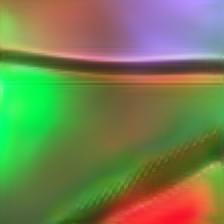
\includegraphics[width=1.05cm]{assets/tactile_sim.png}};
\node[lab] at (.6,4.73) {Tactile};
\node[inner sep=0] (iv) at (.6,3.8) {
\includegraphics[width=1.05cm]{assets/rgb_sim.png}};
\node[lab] at (.6,3.1) {RGB};
\node[box,fill=tac!9,draw=tac,text width=1.65cm] (et) at (2.45,5.45) {\textbf{Tactile encoder}\\SITR-B/16};
\node[box,fill=vis!9,draw=vis,text width=1.65cm] (ev) at (2.45,3.8) {\textbf{Visual encoder}\\MAE-L/16};
\node[lab,fill=white,text=vis,inner sep=1pt] at ($(et.north)+(0,.13)$) {FROZEN};
\node[lab,fill=white,text=vis,inner sep=1pt] at ($(ev.north)+(0,.13)$) {FROZEN};
\draw[a] (it)--(et); \draw[a] (iv)--(ev);

% Tokens are drawn separately from operations.
\tokens{5.00}{5.50}{tac}
\filldraw[fill=tac!65,draw=tac,line width=.4pt] (6.25,5.50) rectangle +(.16,.22);
\node[lab] at (5.7,5.10) {$Q_0$: 196 spatial + 1 pose};
\draw[a,draw=tac] (et.east)--node[lab,above] {Linear\\$768\!\to\!768$}(4.90,5.45);
\tokens{5.00}{3.85}{vis}
\node[lab] at (5.7,3.45) {$M$: 197 visual tokens};
\draw[a,draw=vis] (ev.east)--node[lab,above] {Linear\\$1024\!\to\!768$}(4.90,3.8);

% Taps from different depths have identical spatial resolution.
\foreach \x in {4.85,5.30,5.75,6.20}{\gridmap{\x}{6.80}{tac}}
\node[lab] at (5.7,7.40) {Four intermediate taps $T_i$};
\node[lab] at (5.7,6.55) {Blocks 3, 6, 9, 12};
\draw[a,draw=tac] (et.north east) |- (4.7,6.98);
\node[box,draw=bn,fill=bn!7,text width=1.85cm] (inject) at (8.85,6.98) {\textbf{Gated injection}\\per tap; panel (c)};
\draw[a,draw=tac] (6.7,6.98)--(inject.west);
\node[box,draw=out,fill=out!7,text width=1.85cm] (dpt) at (12.10,6.98) {\textbf{DPT decoder}\\Reassemble + fuse};
\draw[a] (inject)--(dpt);
\node[inner sep=0] (dep) at (15.65,7.02) {
\includegraphics[width=.86cm]{assets/depth_gt.png}};
\node[inner sep=0] (nor) at (17.1,7.02) {
\includegraphics[width=.86cm]{assets/normal_gt.png}};
\node[lab] at (15.65,6.39) {Depth}; \node[lab] at (17.1,6.39) {Normals};
\draw[a] (dpt.east)--(14.1,6.98)--(14.1,7.65)-|(dep.north);
\draw[a] (14.1,7.65)-|(nor.north);

% Compact trunk overview; detailed information flow appears below.
\filldraw[draw=bn!35,fill=bn!4,rounded corners=3pt,line width=.6pt] (7.32,3.68) rectangle (10.55,5.85);
\node[align=center] at (8.93,5.51) {\textbf{Asymmetric fusion}\\4 layers; panel (b)};
\tokens{8.30}{4.74}{bn}
\node[lab] at (8.93,4.44) {16 bottleneck tokens};
\node[lab] at (8.93,4.01) {Read $M$; update $Q_\ell$, $B_\ell$};
\draw[a,draw=tac] (6.55,5.45)--(7.32,5.45);
\draw[a,draw=vis] (6.45,3.9)--(7.0,3.9)--(7.0,4.4)--(7.32,4.4);
\draw[ctx] (8.85,5.85)--node[lab,right,fill=white,inner sep=1pt] {$B_4$}(inject.south);
\node[box,draw=out,fill=out!7,text width=2.2cm] (pose) at (12.65,4.78) {\textbf{Pose head}\\Concat + MLP};
\draw[a] (10.55,4.78)--node[lab,above] {$Q_4$}(pose.west);
\node[lab] at (12.65,3.80) {Pose token $\Vert$ mean spatial\\$768+768=1536$};
\node[align=center] (se) at (16.5,4.78) {\textbf{Planar pose}\\$(\cos\theta,\sin\theta,t_x,t_y)$};
\draw[a] (pose.east)--(se.west);
\node[lab,anchor=east] at (17.8,3.1) {Token width: 768\quad\textcolor{tac}{\rule{6pt}{6pt}} Tactile\quad\textcolor{vis}{\rule{6pt}{6pt}} Visual\quad\textcolor{bn}{\rule{6pt}{6pt}} Bottleneck};
\draw[ink!25,line width=.5pt] (.1,2.84)--(17.9,2.84);

% Fusion detail: attention query enters from the left; context from above.
\node[title] at (.1,2.55) {(b) One fusion layer $\ell$};
\node[lab,anchor=west] (m) at (.2,1.98) {$M$ (read-only)};
\node[box,draw=bn,fill=bn!7,text width=1.45cm,minimum height=.5cm] (cb) at (3.55,1.98) {Cross-attn};
\node[lab] (bprev) at (3.55,1.30) {$B_{\ell-1}$};
\draw[a] (bprev)--(cb.south);
\draw[a,draw=vis] (m.east)--node[lab,above] {K,V}(cb.west);
\node[lab] (bl) at (5.35,1.98) {$B_\ell$};
\draw[a,draw=bn] (cb)--(bl);
\draw[a,draw=bn] (bl.east)--(8.4,1.98);
\node[lab,anchor=west] at (8.4,1.98) {carry to layer $\ell+1$};
\node[lab] (qp) at (.8,.88) {$Q_{\ell-1}$};
\node[box,draw=bn,fill=bn!7,text width=1.55cm] (cq) at (5.35,.88) {Cross-attn\\FFN};
\node[box,text width=1.55cm] (sa) at (8.1,.88) {Self-attn\\FFN};
\node[lab] (ql) at (10.05,.88) {$Q_\ell$};
\draw[a] (qp)--node[lab,above] {queries}(cq);
\draw[a,draw=bn] (bl)--node[lab,right] {K,V}(cq);
\draw[a] (cq)--(sa); \draw[a] (sa)--(ql);
\node[lab,anchor=west] at (.15,.12) {Attention and FFN include pre-normalization and residuals; $B_0$ is learned.};
\draw[ink!25,line width=.5pt] (11.0,.08)--(11.0,2.65);

% Explicit gated residual, separate from the trunk query stream.
\node[title] at (11.3,2.55) {(c) Visual injection at tap $i$};
\node[lab] (tt) at (11.7,1.32) {$T_i$};
\node[box,draw=bn,fill=bn!7,minimum width=1.4cm] (ca) at (13.55,1.32) {Cross-attn};
\node[lab] (bb) at (13.55,2.13) {$B_4$};
\draw[ctx] (bb)--(ca);
\node[draw=bn,circle,inner sep=1.5pt] (mul) at (15.25,1.32) {$\times$};
\node[draw=ink!70,circle,inner sep=1.5pt] (add) at (16.65,1.32) {$+$};
\node[lab] (tp) at (17.65,1.32) {$T'_i$};
\draw[a] (tt)--(ca); \draw[a] (ca)--(mul); \draw[a] (mul)--(add); \draw[a] (add)--(tp);
\draw[a] (12.15,1.32)--(12.15,.39)--(16.65,.39)--(add.south);
\fill[ink!80] (12.15,1.32) circle (.035);
\node[lab] (alpha) at (15.25,2.12) {$\alpha_i$};
\draw[a] (alpha)--(mul);
\node[lab,anchor=west] at (11.3,.04) {Independent parameters per tap; $\alpha_i$ starts at zero.};
\end{tikzpicture}
\end{document}
